% /* Notes
% (TODO: the address on the deice is diferent)
% Alloc: just allocate on device, uninitialized
% to: map to device before execution
% from:  map from device after execution
% tofrom: map to and from
% https://www.appentra.com/about-us/
% */
OpenMP is a widely used directive-based parallel programming
model, that now supports offloading computations from hosts to device 
accelerators. 
% which offers accelerator programming and supports heterogeneous
% computing systems with host CPUs and device accelerators (currently
% GPUs and FPGAs) from version 4.0 onwards.  
Notable accelerator-related features 
in OpenMP 4.5 include unstructured data
mapping, asynchronous execution, and runtime routines for device
memory management. 
% \vspace{-10pt}
\subsubsection{OMP 4.5 Target offloading and Data mapping}
OMP 4.5 offers the \textit{omp target} directive 
for offloading computations to devices and the \texttt{omp target data}
directive for mapping data across the host and the corresponding
device data environment.
% is used to generate a target 
% task that can be offloaded to a device, and also to map variables 
% to the device data environment. 
% The \textit{omp target data} directive explicitly maps variables 
% from a host environment to a device data environment.
On heterogeneous systems, managing the movement of data between the host and the device can be challenging, and is often a major source of performance and correctness bugs. 
In the OpenMP accelerator model, 
% hosts and devices have their own memory space – i.e., data environments – and 
data movement between device and host 
is supported either explicitly via the use of a \texttt{map} clause 
or, implicitly through default data-mapping rules. 
The optimal, or even correct, specification of map clauses can be non-trivial and error-prone because it requires users to reason about the complex dataflow analysis. 
% To ensure that the map clauses are correct, OpenMP programmers 
% need to identify statements 
% that define variables involved in target clauses, and
% each definition of such a variable to all the uses that can be 
% reached by it in the program.
% Given a data map construct, its semantics depends on all the previous usages of the map construct.
% Therefore, dataflow analysis of map clauses is necessarily 
% context-sensitive since the entire call sequence leading up to a specific 
% map construct can impact its behavior.
% 
% Therefore, it is context sensitive and the entire call sequence leading up to the construct impacts its behavior.
% On heterogeneous systems, managing the 
% movement of data between the host and the 
% the data movement between host and device is
% a common performance and energy efficiency bottleneck, as well as a
% major source of performance and correctness bugs.  In the OpenMP
% accelerator model, host and device have their own memory space --
% i.e., data environment -- and the data movement is supported by the
% explicit data copy via \texttt{map} clause or, implicitly through 
% default \texttt{map} rules.
% The optimal, or even
% correct specification of \texttt{map} clause is non-trivial and 
% error-prone because it requires element-wise dataflow analysis to
% identify the statements/instructions that define the value at given
% program points and variables/array elements.
% Even given an existing application that uses the 
% target offloading feature, understanding the data mapping 
% behavior is nontrivial. 
% Given a data map construct, its semantics depends on all the previous 
% usages of the map construct. Therefore, it is context sensitive and 
% the entire call sequence leading up to the construct impacts its 
% behavior.
\subsection{OpenMP 4.5 Map Semantics}
\autoref{mapSemantics} shows a schematic illustration 
of the complex set of rules used when mapping 
a host variable to the corresponding list item 
in the device data environment, as specified 
in the OpenMP 4.5 standard. For correctness, in this paper 
we assume the device is a GPU, and mapping 
a variable from host to device introduces a host-device memory copy, 
and vice-versa. 
However, the bugs that we identify reflect errors in the OpenMP 
code regardless of the target device. 

The different map types that OpenMP 4.5 supports are, 
\begin{itemize}
\vspace{-5pt}
    \item alloc: allocate on device, uninitialized
 \item to: map to device before kernel execution, (host-device memory copy)
 \item from:  map from device after kernel execution (device-host memory copy)
 \item   tofrom: copy in and copy out the variable at the entry and exit of the device environment  
\end{itemize}
\vspace{-9pt}
The default map type for arrays is \textit{tofrom}, 
% that is copy in and copy out the array at the entry and exit of 
% the device enviro nment. 
while the default for scalars
is \textit{firstprivate}, that is the only copy the value of the 
scalar at the entry to the device environment.
\begin{figure}[h!]
% \hspace{-80pt}
\vspace{-20pt}
\begin{subfigure}[b]{1\textwidth}
\centering
    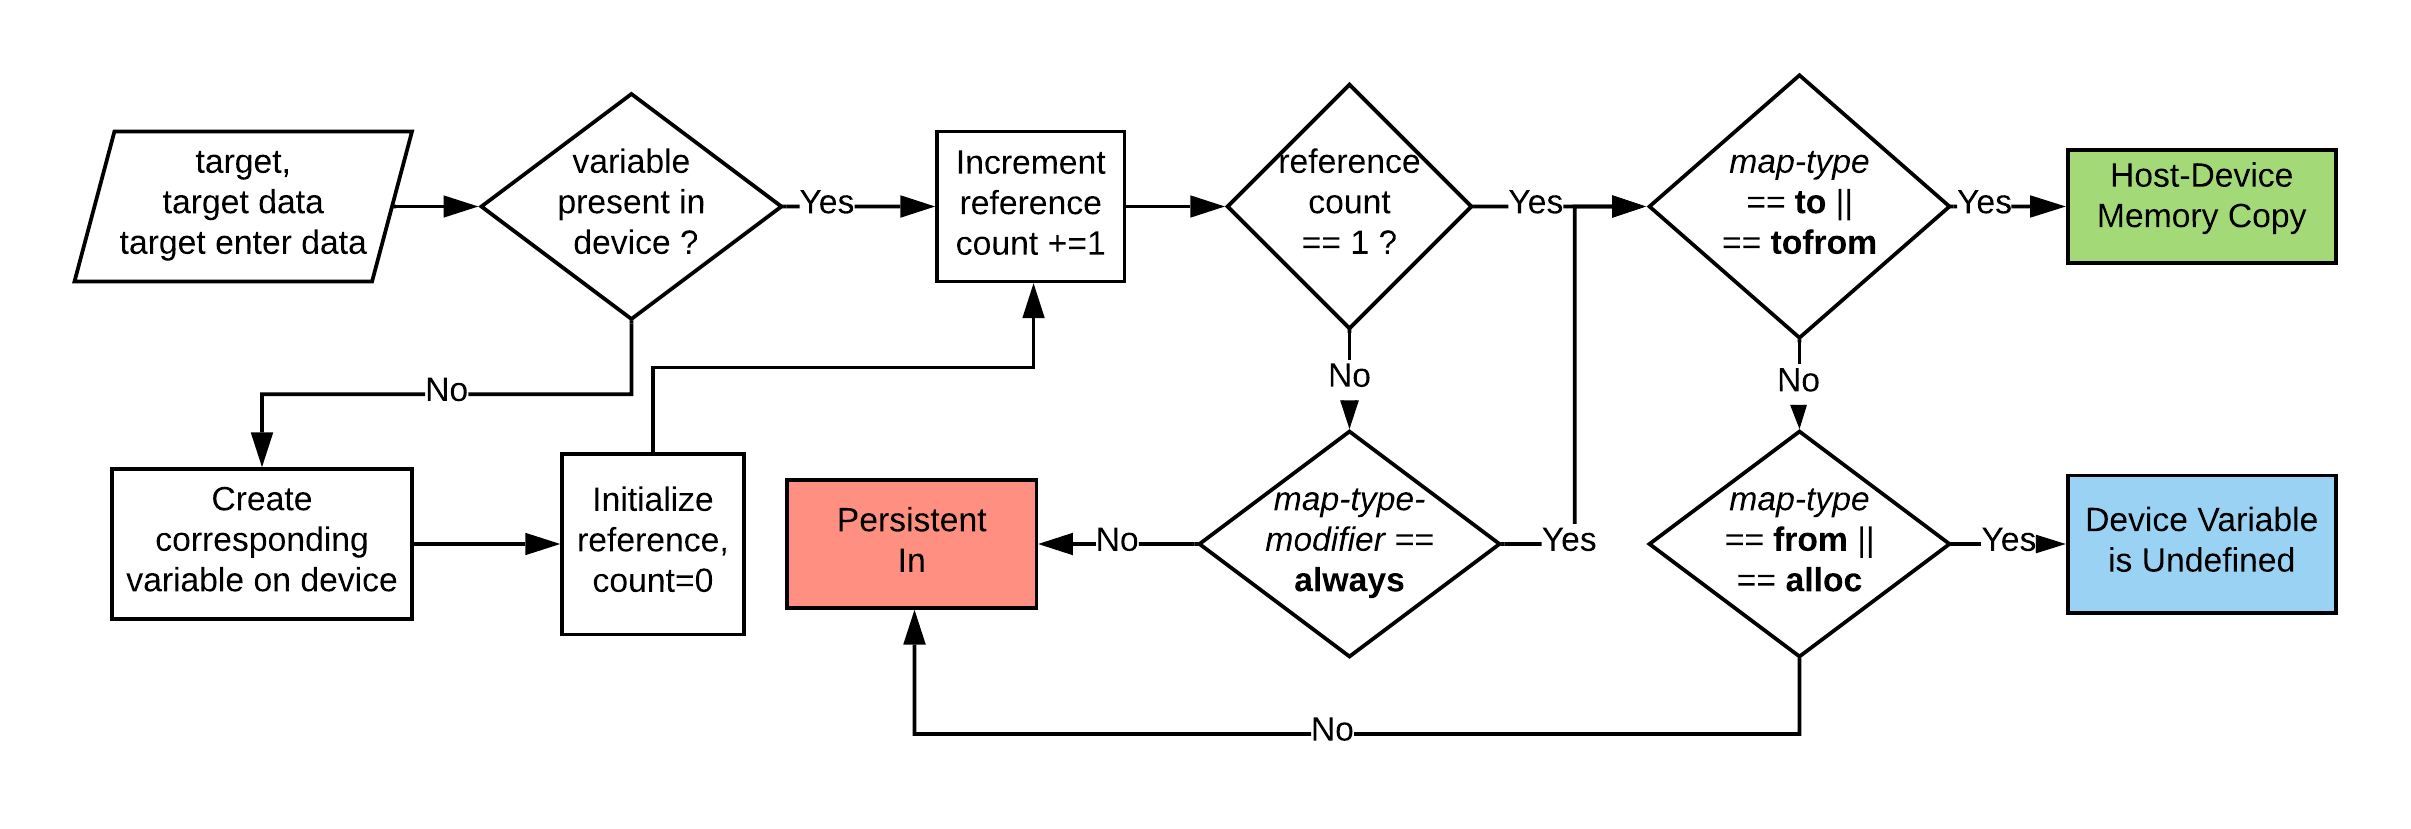
\includegraphics[scale=0.6]{images/data-enter.png}
  \caption{Flowchart for Enter Device Environment}
    \label{host-device-flowchart}    
  \end{subfigure} 
  
%   \hspace{20pt}
  \begin{subfigure}[b]{1\textwidth}
  \centering
    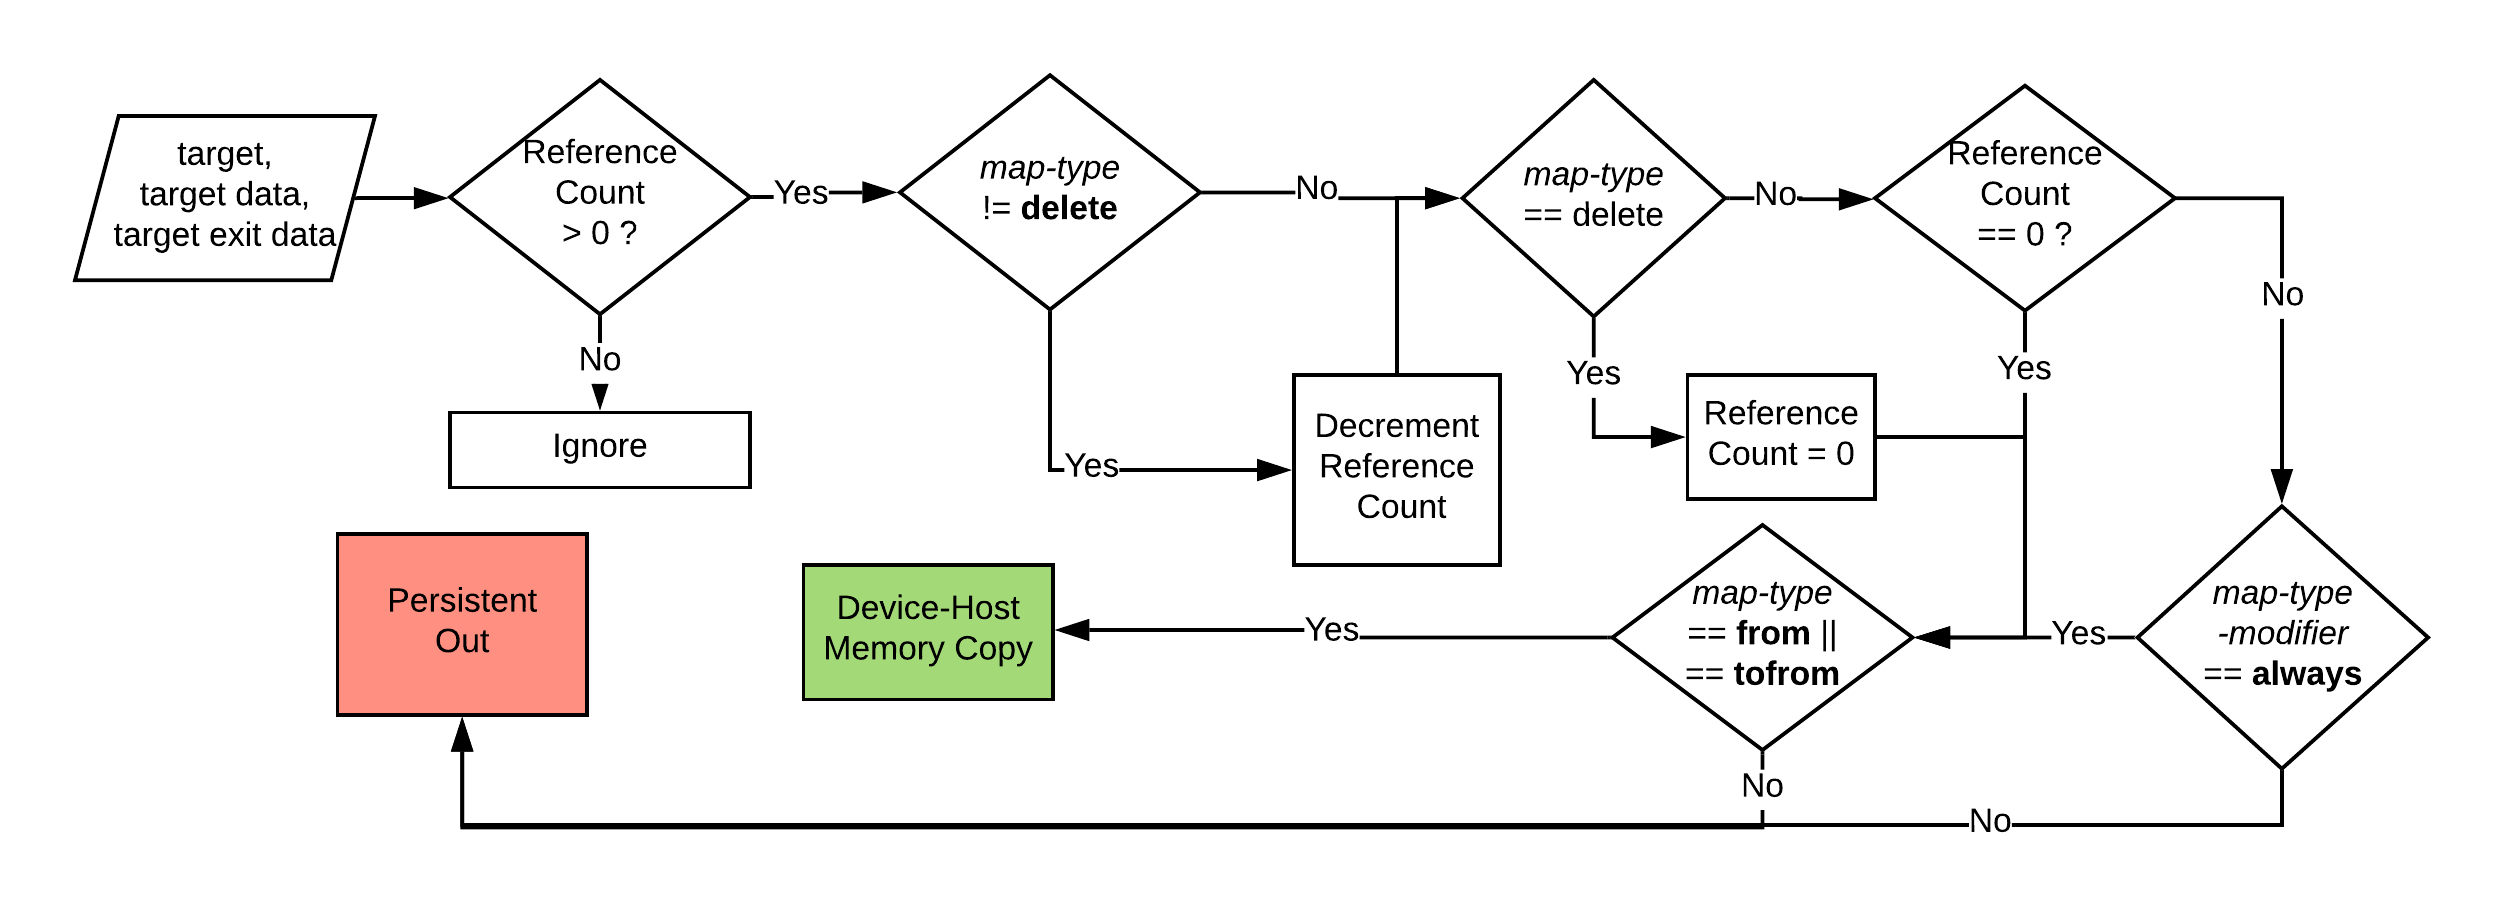
\includegraphics[scale=0.6]{images/data-exit.png}
    \caption{Flowchart for Exit Device Environment}
    \label{device-host-flowchart}    
  \end{subfigure}
  \caption{Flowcharts to show how to interpret the map clause}    
  \label{mapSemantics}
%   \vspace*{-10pt}
\vspace{-20pt}
\end{figure} 
% The OpenMP 4.5 specification specifies the semantics of the \textit{map}
% clause, and \autoref{mapSemantics} illustrates how the spec 
% interprets the data map constructs. 
% The flowchart also motivates our argument that understanding the \textit{map} clause is not trivial, it 
%  shows the complex set of rules defined in the OpenMP 4.5 spec, 
% that is used to determine how to map a  host variable to the corresponding list item in the device data environment.
% We make a simplifying assumption that the CPU host is the current 
% task's data environment and the device is a GPU, and hence the mapping from the host to the device
% refers to the Device-Host and Host-device memory copy.
As \autoref{mapSemantics} shows, OpenMP 4.5 specification uses the reference count of a variable, to decide when to introduce 
a device/host memory copy. The host to device memory copy is 
introduced only when the reference count is incremented from 0 to 1 and the ``to'' attribute is present. 
Then the reference count is incremented every time a 
new device map environment is created. 
The reference count is decremented on encountering a ``from'' or ``release'' 
attribute, while exiting the data environment. 
Finally, when the reference count is decremented to zero from 1, and the 
``from'' attribute is present, 
the variable is mapped back to the host from the device.
% \autoref{statemachine} shows an example state machine, 
% to decide when to insert the memory copies.
% \begin{figure}
% %  \hspace*{-30pt}
%     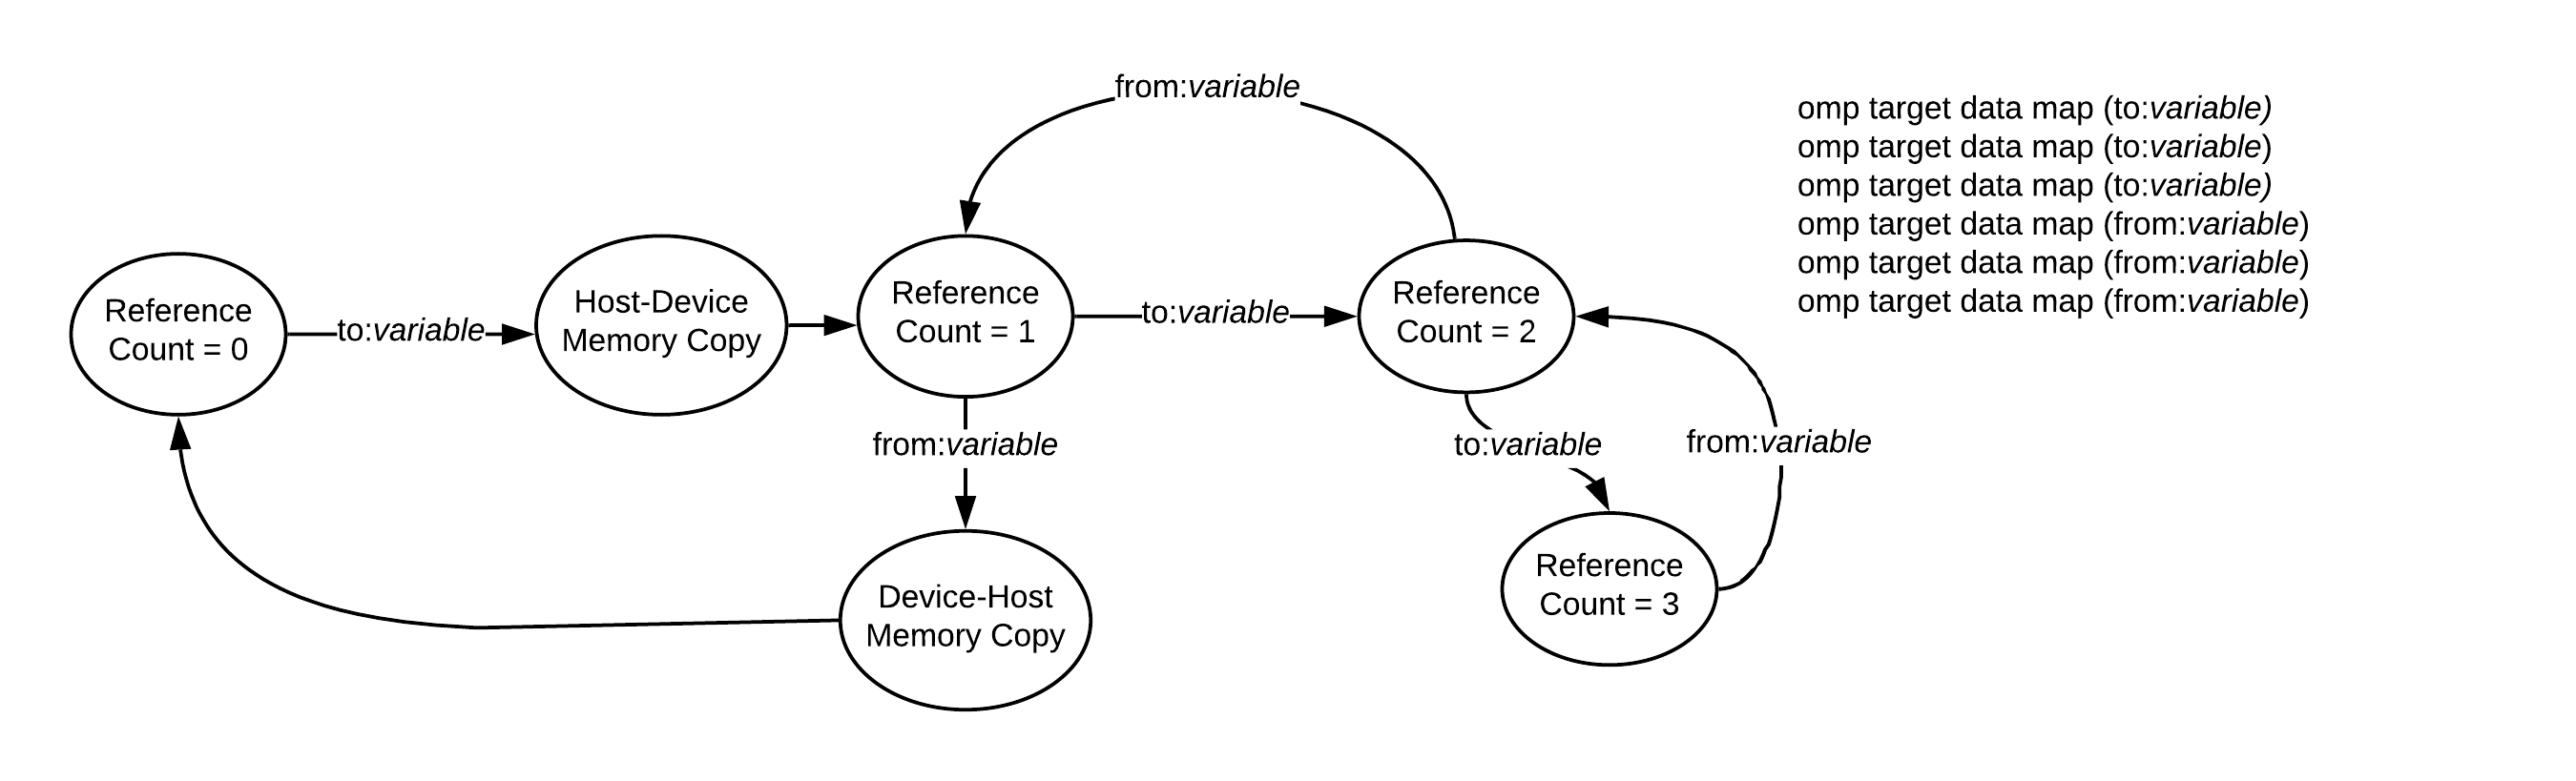
\includegraphics[scale=0.6]{images/statemachine.png}
%     \caption{State Machine for inserting Host/Device Memory Copies } \label{statemachine}
% \end{figure}
\vspace{-10pt}
\subsection{Our Solution}
% \vspace{-50pt}
To address the complexity of using OpenMP's target map 
clauses, we propose a static analysis 
tool called OmpSan to perform OpenMP code ``sanitization''.
OmpSan is a compile-time tool, which does static verification 
of data mapping constructs based on a dataflow analysis.
The key principle guiding our approach is that, ``An OpenMP program is expected to yield the same result when enabling
or disabling OpenMP constructs''.
% this issue as first-aid error detection, we propose a
% compile-time approach based on dataflow analysis. 
% The key principle guiding our error detection approach is that
% ``A user program yields the same result when enabling or disabling
% OpenMP constructs''.
% \footnote{With the exception of privatization clauses, which is unrelated to our goal, and beyond the scope of this work}.
Our approach detects errors by comparing 
dataflow information (reaching definitions via
LLVM's memory SSA representation \cite{llvm-memoryssa-url}) 
between the OpenMP and baseline code.  We developed an
LLVM-based implementation of our approach and evaluated its
effectiveness using several case studies.
Our major contributions include the fo1llowing.
\begin{itemize}
\vspace{-3pt}
\item An algorithm to analyze OpenMP runtime library calls inserted by Clang in the LLVM IR, to infer the host/device memory copies. We expect 
that this algorithm will have applications beyond our OmpSan tool. 
% according to OpenMP 4.5 semantics
\item A static analysis technique to validate if the host/device memory copies respect the original memory def-use relations. 
% \item Reporting error/warnings on usage of data mapping constructs 
% on given user programs
\item Diagnostic information to understand how the map clause affects the 
host and device data environment. 
\end{itemize}\vspace{-10pt}
The paper is organized as follows. 
\autoref{s2} provides certain motivating examples, 
that show common issues  and difficulties in usage of 
OpenMP's \textit{data map} construct. 
\autoref{s03} provides the background information 
that we use in our analysis.
\autoref{s3} presents an overview of our approach to validate 
the usage of data mapping constructs. 
\autoref{s4} presents the LLVM implementation details, and 
\autoref{s5} presents the evaluation and some case studies. 
\autoref{limitation} also lists some of the limitations of 
our tool, some of them common to any static analysis.  
% According to the OpenMP 4.5 semantics, the \texttt{target}, 
% \texttt{target data}, and the \texttt{target enter data} 
% constructs maps host variables to a device data environment. Essentially 
% for the GPU, it inserts host-device and device-host memory copies. 
% The \texttt{map} clause is used to specify how a variable is mapped 
% from the host to the device environment.
